% \tableofcontents
% ========================================================
% DIGITAL READOUT
% ========================================================
\section{Digital Readout of the Analogue Chip}
Initially the analogue chips were read out with an \ac{ATB} and a software called ``psi46expert''. As already mentioned in \ar{sdtb} the \ac{DTB} has some advantages compared to the \ac{ATB}, which was the reason for switching to the \ac{DTB} controlled by the pXar core libraries. In order to be able to accomplish that, an extension to the pXar core was added by the pXar community that is able to process the data of the analogue \ac{ROC}. The extension includes the decoder described in \ar{sdec} and adds all missing \ac{DAC}s to the library. In addition it utilises the \ac{ADC} of the \ac{DTB}.
% ========================================================
\subsection{Functioning Check}
In order to read out an analogue chip with the \ac{DTB}, first of all the basic functioning should be checked. One has to ascertain that the \ac{DUT} is working\footnote{Working in this context means that it is possible to successfully readout calibrate signals} and that is has a set of appropriate \ac{DAC}s for an analogue \ac{ROC}. For the test board parameter file it is best to use the following lines which were found to be good starting values for the \ac{DTB}:\s
{\ubuntu
\begin{tabular}{llr}
	0	&   clk	&  4\\
	1	&	ctr	&  4\\
	2	&	sda	&  19\\
	3	&	tin	&  9
\end{tabular}}\no\s
For the other necessary files the default files from the Perl script (q.v. \ar{srunpx}) suffice. In the next step the python \ac{CLI} can be started; using the version ``CLIX.py'' simplifies matters a lot.\\
Once the \ac{CLI} is running it has to be checked that the \ac{ROC} is responding and programmable, which can be done by reading out its analogue supply current:
\begin{itemize}
	\tri getTBia
\end{itemize}
The \ac{ROC} is programmable if the current is roughly around $24\,$mA and bigger than $5\,$mA. If this is not the case the test board setting sda is probably incorrect. To resolve it one has to do a scan \textit{sda} (adding $\pm5$ to all test board settings) and repeat the measurement until the \ac{ROC} draws current.
% ========================================================
\subsection{\ac{DTB} Timing}
Since the analogue to digital conversion from the signal of the chip is done within the \ac{DTB}, the exact time when to start and stop sampling the signal are uncertain. The information of the data stream will arrive some time after the token was sent and will end some time after it was received again. These timings can be set by two internal delays of the test board:
\begin{description}
	\item[tindelay:] The time after the token was sent from the \ac{DTB} to the \ac{ROC}. 
	\item[toutdelay:] The time after the token was received from the \ac{DTB}.
\end{description}
The whole process is illustrated in \ar{pdelays}. In order that the decoder can work properly the data has to start with an \ac{UB} level and has to stop with the pulse height of the last pixel hit\footnote{If there is no pixel information within the data, the last level has to be \ac{LD}}. The delays are independent from the length of the data stream, because this length also determines the time in between tin and tout. 
\subsubsection{Finding the delays}
First of all it has to be guaranteed that the pixels can be read out at all by checking the raw data. In order to see the data at all tindelay has to be short enough and toutdelay has to be long enough, s.t. the data is inside the readout window: $5$ and $20$ were found as good starting values. It is advantageous to look at the pixel with the address $5$ $12$ because it includes all $6$ different address levels.\s
\begin{minipage}{5.5cm}
	\begin{itemize}\ubuntu
		\item[$\triangleright$] set\_tb\_delay tindelay 5
		\item[$\triangleright$] set\_tb\_delay toutdelay 20
	\end{itemize}
\end{minipage}
\schema[close]{\vspace*{1.1cm}}{\schemabox{\ubuntu$\triangleright$\hspace*{2pt} set\_tin\_tout 5 20 \footnotemark[3]}}
\footnotetext[3]{The functions behind the curly brackets are short versions from CLIX.py}
\no\s
\begin{minipage}{4.2cm}
	\begin{itemize}\ubuntu
		\tri maskAllPixels 1
		\tri testAllPixels 0
		\tri maskPixel 5 12 0
		\tri testPixel 5 12 1
	\end{itemize}
\end{minipage}
\schema[close]{\vspace*{2.5cm}}{\schemabox{\ubuntu$\triangleright$\hspace*{2pt} enableOnePix 5 20}}
\no\s
\begin{minipage}{4.2cm}
	\begin{itemize}\ubuntu
		\tri daqStart 
		\tri daqTrigger 1 500
		\tri dawGetRawEvent
		\tri daqStop
	\end{itemize}
\end{minipage}
\schema[close]{\vspace*{2.5cm}}{\schemabox{\ubuntu$\triangleright$\hspace*{2pt} daqRawEvent}}\no\s
An example readout looks like this:
\termi{[-3, -19, -9, -193, -1, 96, -55, 58, 108, 164, 212, 93, -4, -6]}
The values slightly below $0$ in the beginning and the end of the example correspond to the zero line of the analogue signal. In between is the \ac{ROC} header and the pixel information. For this example one would have to increase \textit{tindelay} by $3$ and decrease \textit{toutdelay} by $2$ in order to get ride of the base line values. If the pixel information is missing, the delay of the calibration is probably wrong and one has to shift the \ac{DAC} \textit{caldel} by orders of $10$ in both directions until the information appears.
\begin{itemize}
	\tri \ubuntu setDAC caldel <\textit{n}>
\end{itemize}\no\par
During these tests I noticed that the \ac{PG} was set up 
\begin{wrapfigure}{r}{4cm}
	\vspace*{-10pt}
	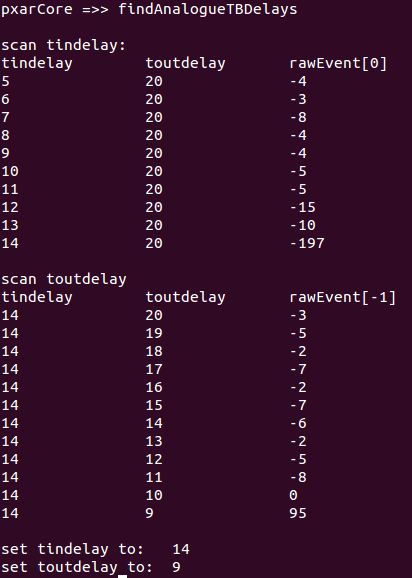
\includegraphics[width=3.9cm]{findDelay}
	\caption{Example output of findAnalogueTBdelays.}
	\label{pfinddel}
	\vspace*{-5pt}
\end{wrapfigure} 
incorrectly, as the delay between the calibrate and the trigger was set to a fixed value allowing only a  \textit{wbc} of $100$. I fixed that by making the delay dependent on the \textit{wbc} set in the dacParameter file.\\
Once the data is read out correctly and the pixel information is shown one can start adjusting the test board delays. In order to accomplish that function:
\ubu{findAnalogueTBdelays} 
was implemented, which adjusts them automatically. First of all it will activate a single pixel and mask and disable the rest. Then it will increase tindelay from $5$ until the first word in the data stream has a value lower than $-100$, which usually corresponds to \ac{UB}. Afterwards it will decrease toutdelay starting from $20$ until the last word is bigger than $20$, which corresponds to the \ac{PH}. Finally it will print out and set the correct values. An example of its complete output is shown in \ar{pfinddel}. Raw events now should look like this:
\termi{[-196, 0, 97, -54, 57, 106, 164, 212, 91]} 
In order to permanently save the values and start the \ac{DTB} with them per default the following lines have to be added to the tbParameter.dat file:\s
{\ubuntu
\begin{tabular}{llr}
	247	&   tindelay	&  <\textit{found value}>\\
	248	&	toutdelay	&  <\textit{found value}>
\end{tabular}}\no\s
\begin{figure}[ht]
	\centering
	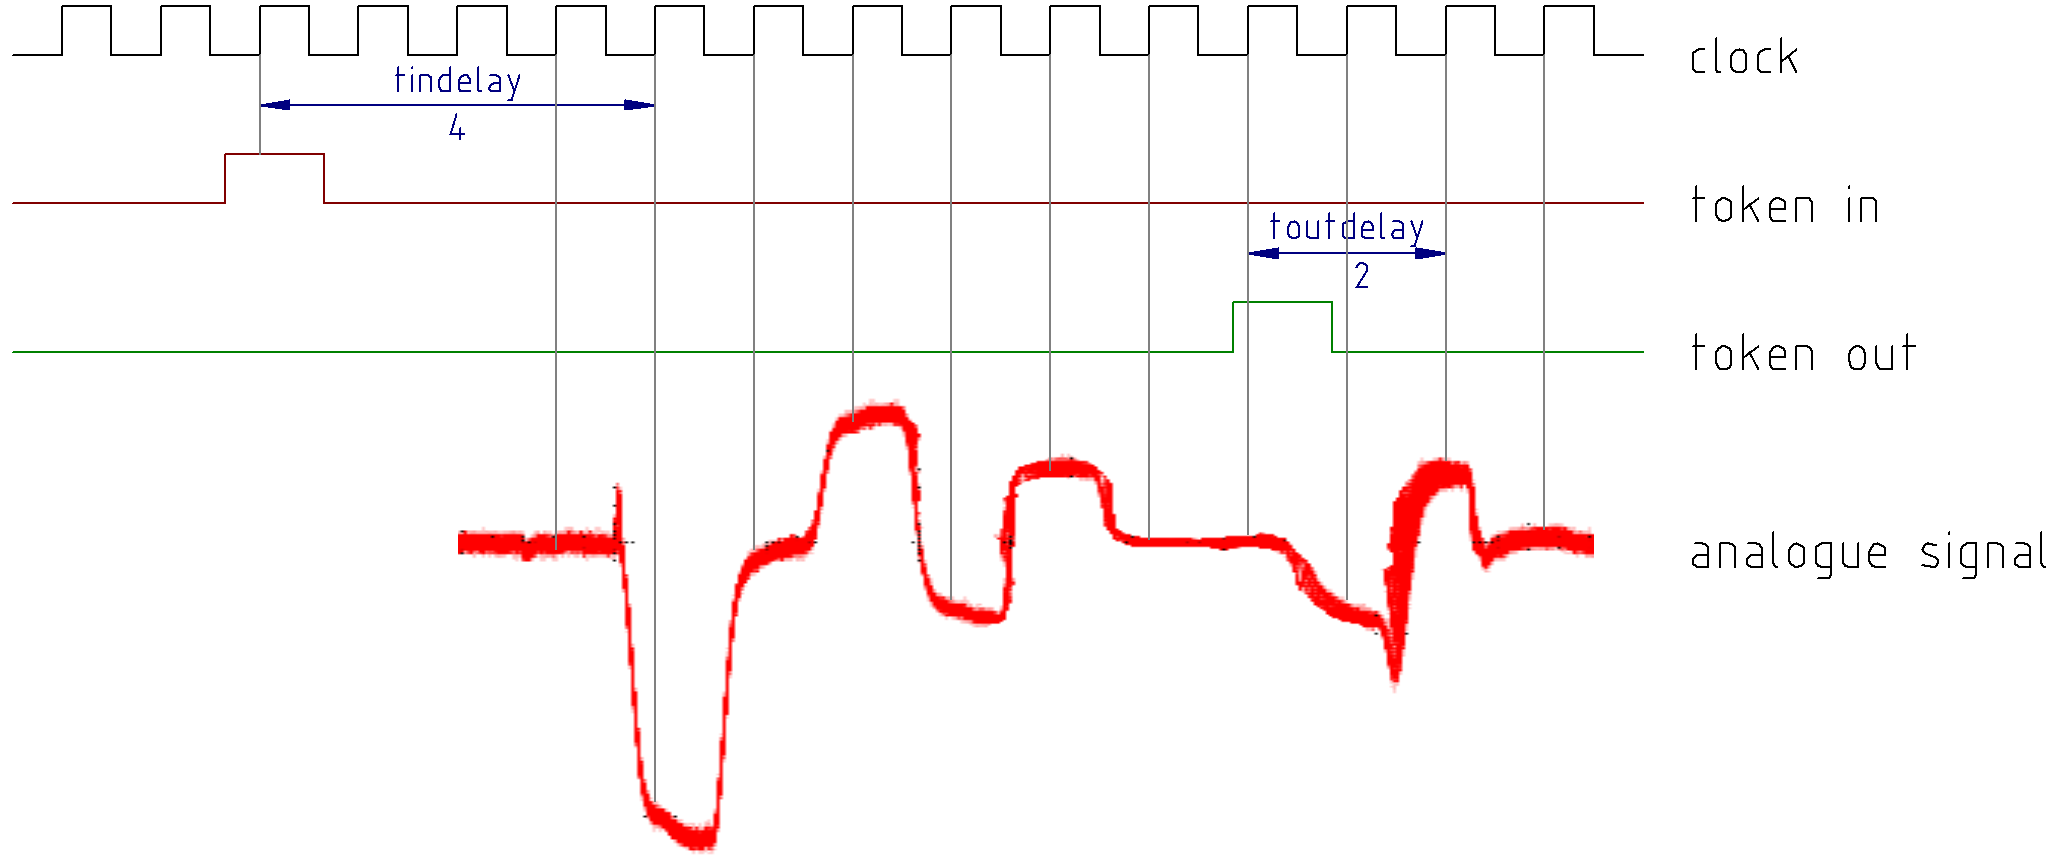
\includegraphics[width=0.95\textwidth]{tbdelays}
	\caption{Demonstration of the test board delays. The clock is always sampling at the rising edge.}
	\label{pdelays}
\end{figure}\no
% ========================================================
\subsection{Sampling Point of the \ac{ADC}}
As one can see in \ar{pdelays} the analogue signal is no rectangular wave. If two levels with different values follow each other the latter one takes some time until it is stable. This behaviour is illustrated in \ar{pdel2}. That is why it important to shift the sampling point of the \ac{ADC} to a sweet spot where the level is stable. In order to accomplish that, the delay of the internal clock has to be adjusted. A wrong sampling point will shift the current level depending on the previous or following one (depending on the position).\\
To find the best delay I implemented the function:
\ubu{find\_clk\_delay} 
for the \ac{CLI}, which will do the following: First it will activate six special pixels that have level sequences $0\rightarrow 2 \rightarrow 0$, $1\rightarrow 2 \rightarrow 1$, $\hdots$, $5\rightarrow 2 \rightarrow 5$ within their pixel addresses\footnote{E.g. the pixel $0$ $44$ decodes to the address levels $0$ \textbf{$0$ $2$ $0$} $0$.}. It will then measure and average the values of the middle address ($2$) for each of these pixels for all clock delay settings from $0-24$. This setting is equivalent to a delay in units of nanoseconds. The corresponding values are plotted in \ar{psplits}. For low clock settings the value is split depending on the pixel from what it is measured. Then all lines converge until they split again for high clock delays. In order to find the ideal clock setting, the function first calculates the mean of all six values for a fixed delay and then it determines the average deviation from that mean value. The delay with the smallest deviation is considered the best setting. In the end the function will print the best value and lowest deviations. Following values in the tbParameter.dat file have to be changed for starting the \ac{DTB} with these settings:\s
{\ubuntu
\begin{tabular}{llr}
	0	&   clk	&  4\\
	1	&	ctr	&  4\\
	2	&	sda	&  19\\
	3	&	tin	&  9
\end{tabular}}
$\longrightarrow$
{\ubuntu
\begin{tabular}{lll}
	0	&   clk	&  <\textit{found value}>\\
	1	&	ctr	&  <\textit{found value}>\\
	2	&	sda	&  <\textit{found value}> + 15\\
	3	&	tin	&  <\textit{found value}> + 5
\end{tabular}}\no\s
By shifting the clock the token in and token out signal might be sampled in another cycle. To compensate for that one should run 
\begin{itemize}
	\tri \ubuntu findAnalogueTBdelays
\end{itemize}
again. Find\_clk\_delay will plot a histogram of the address levels for the best clock delay setting. If there are only single, well separated peaks, the delay was successfully set as in \ar{padrlev}
\begin{figure}[ht]
	\centering
	\subbottom[Schematic level shift for the addresses $0\rightarrow x\rightarrow2\rightarrow x\rightarrow0$. It drawn excessively for better demonstration. Every single coloured line corresponds to a different pixel address. The red arrow marks inconvenient sampling points as one can see the level splitting up.]{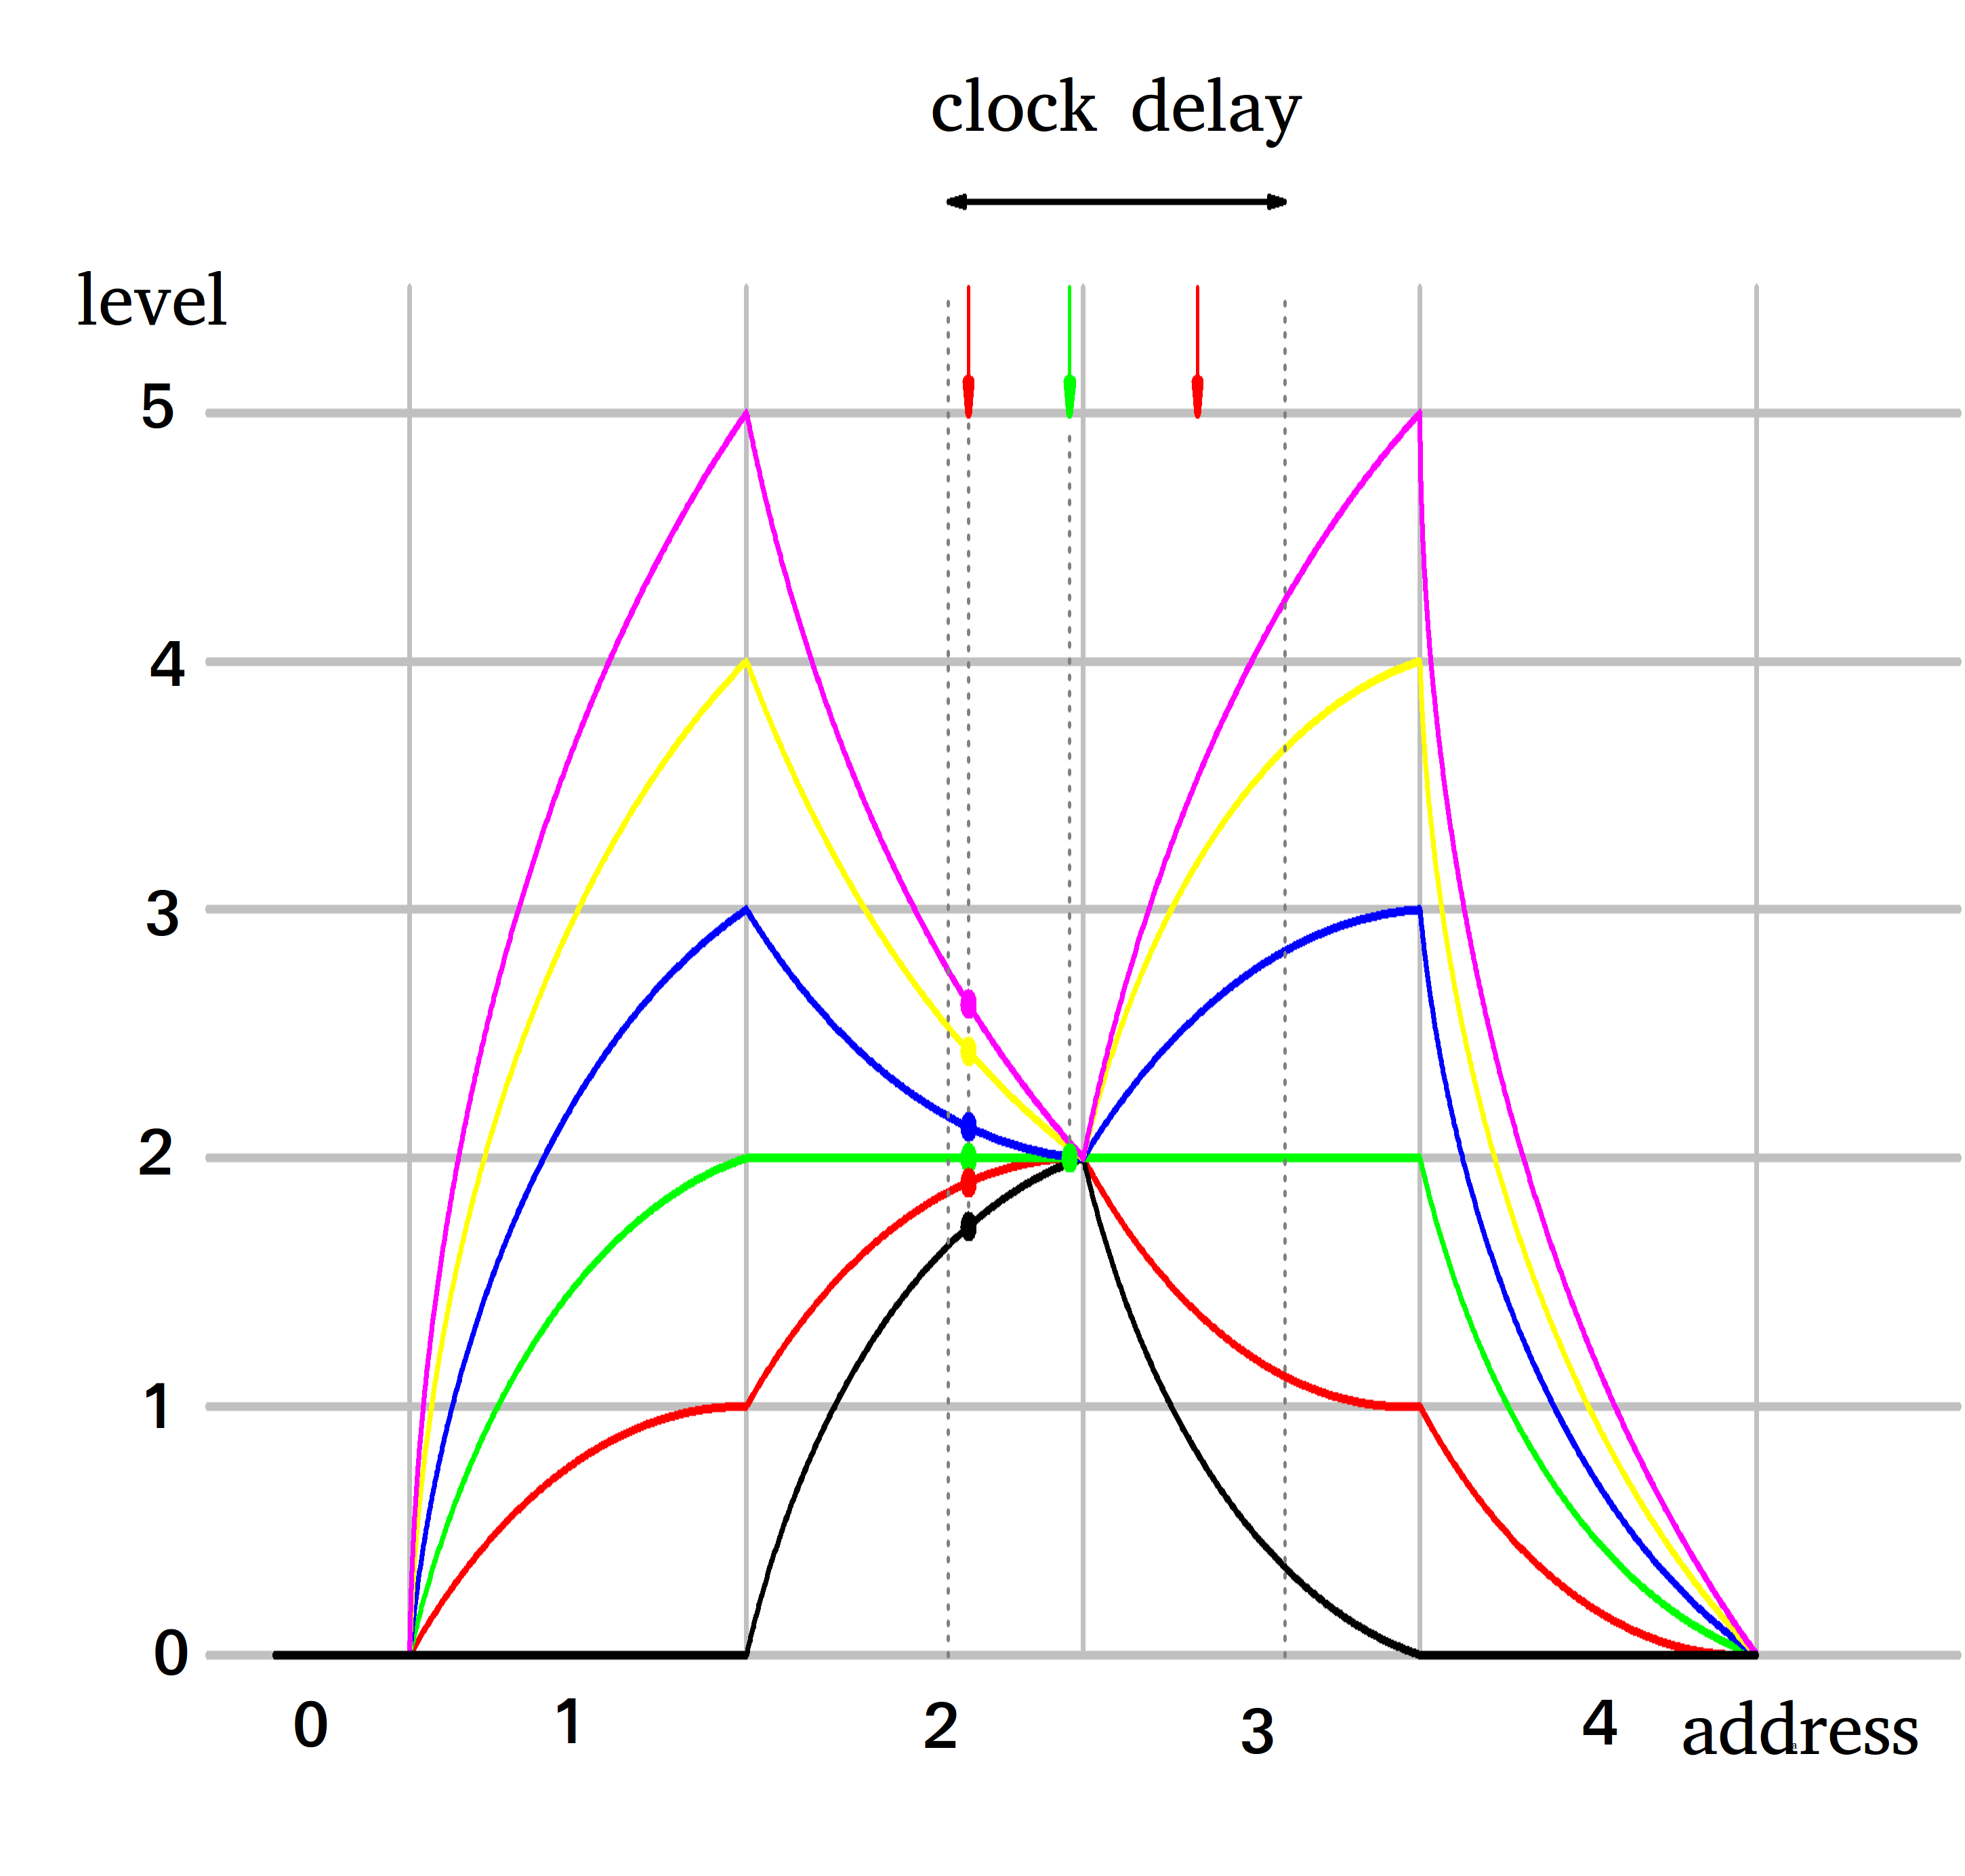
\includegraphics[width=0.47\textwidth]{clkdelay}\label{pdel2}}
	\hfill
	\subbottom[Real level splits measured with the find\_clk\_delay function. The vertical line shows the clock setting with the lowest deviation and the vertical lines demonstrate the decoding window.]{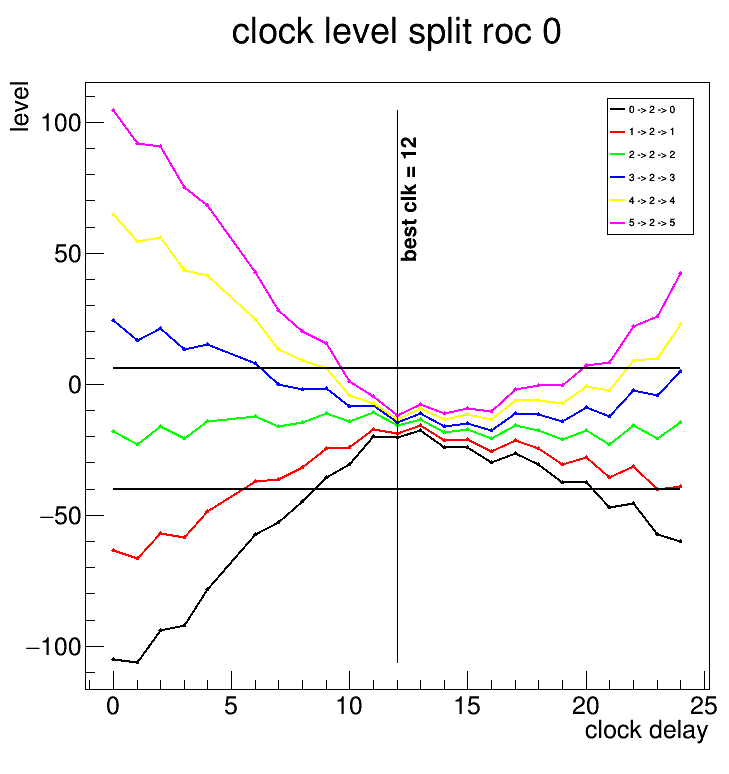
\includegraphics[width=0.47\textwidth]{splits}\label{psplitsreal}}
	\caption{Level splits of the analogue signal.}
	\label{psplits}
\end{figure}\no
\begin{figure}[ht]
	\centering
	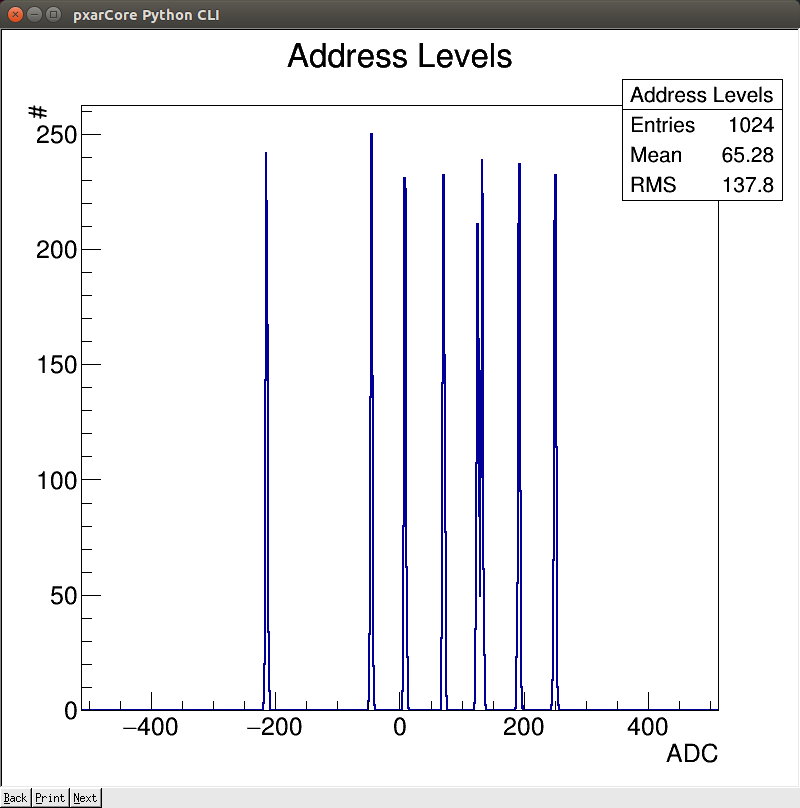
\includegraphics[width=0.5\textwidth]{address_lvls}
	\caption{Address level histogram of thousands hits of the pixel $5$ $12$.}
	\label{padrlev}
\end{figure}\no
% ========================================================
% TRIMMING
% ========================================================
\section{pXar Tests}
Once the timing and the sampling point are set up correctly the \ac{ROC}s may be operated with the full pXar software. The \ac{GUI} has some very useful test functions that help optimising the \ac{ROC} \ac{DAC}s. A picture of the \ac{GUI} with all its tests can be found in \ar{pgui}. The most important ones are quickly sketched in the following:
% ========================================================
\subsection{GainPedestal}\label{sgainped}
The GainPedestal test measures the pulse height curves for ten different \textit{vcal} values $[50, 100, 150, 200, 250, 210, 350, 490, 630, 1400]$ for every single pixel and saves them to the file ``phCalibration\_C<\textit{\ac{I2C}}>.dat'' into the dacParameter directory. These values are important for the pulse height calibration of real pixel data.
\begin{figure}[ht]
	\centering
	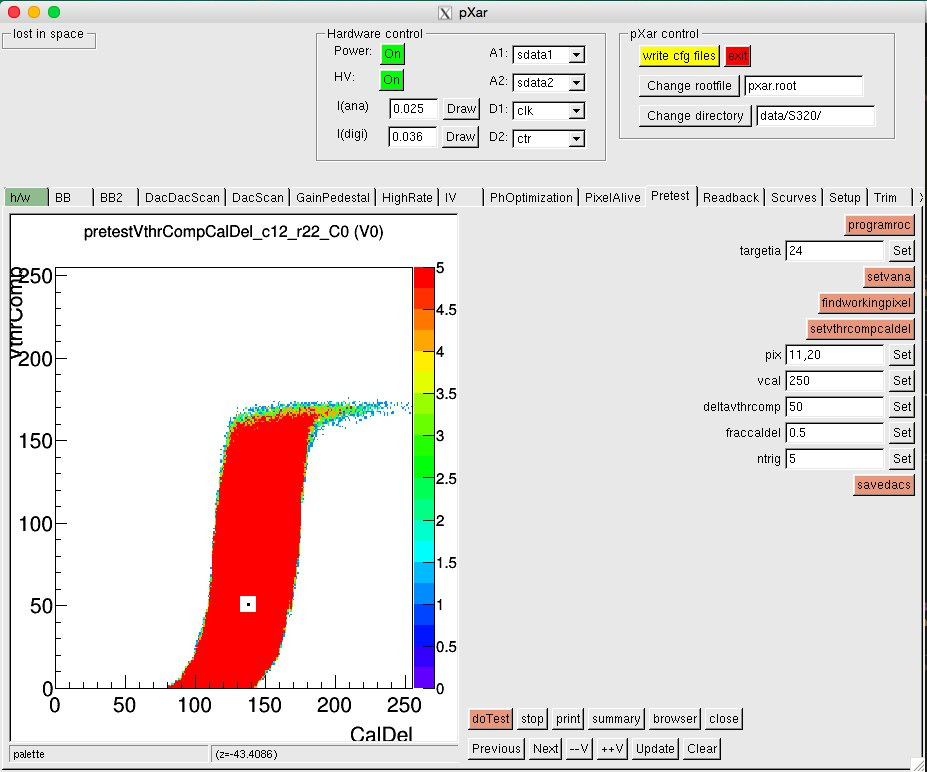
\includegraphics[width=0.95\textwidth]{gui}
	\caption{pXar \ac{GUI}. The tests are shown in the grey tabs.}
	\label{pgui}
\end{figure}\no
% ========================================================
\subsection{DacDacScan}\label{stornado}
The default DacDacScan test counts how often a single pixel can be read out successfully after sending ten triggers for every combination of of the \ac{DAC}s \textit{vcal} and \textit{vthrcomp}. It plots the result in a two dimensional histogram as shown in \ar{ptornado}. The readout is only working within a region that is roughly shaped like a tornado, which is why the plot is usually referenced as ``tornado plots''. The shape is determined by the difference of time signals  need to get to the comparator and the overall threshold of the pixel. 
\begin{figure}[ht]
	\centering
	\subbottom[Tornado plot of an analogue \ac{ROC}]{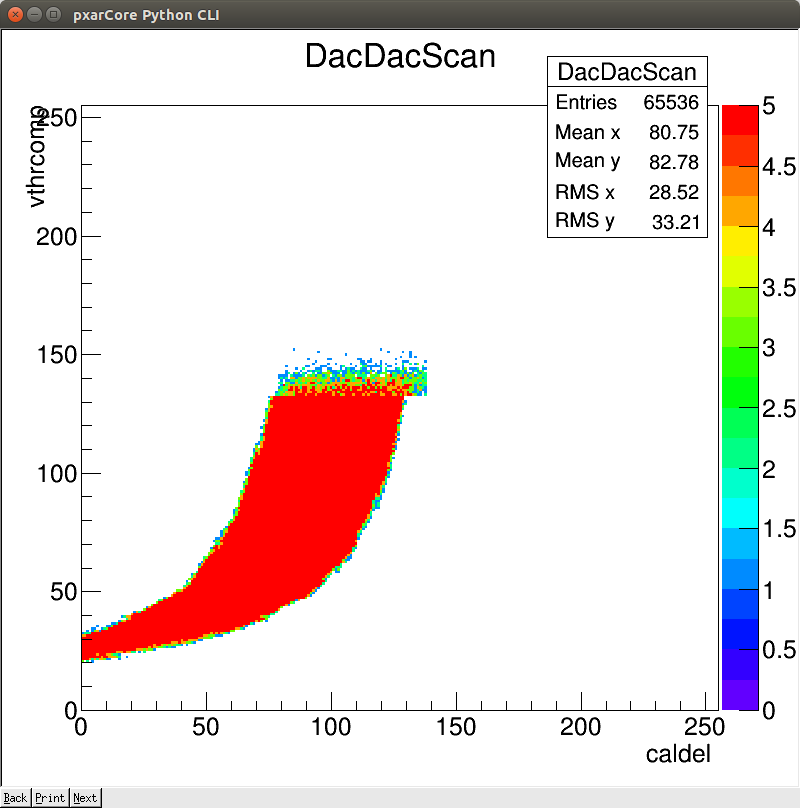
\includegraphics[width=0.47\textwidth]{DacDacScan}\label{ptornado}}
	\hfill
	\subbottom[PixelAlive map. On the top edge are few pixels that do not work at all. Except from that all pixel have 10/10 readouts.]{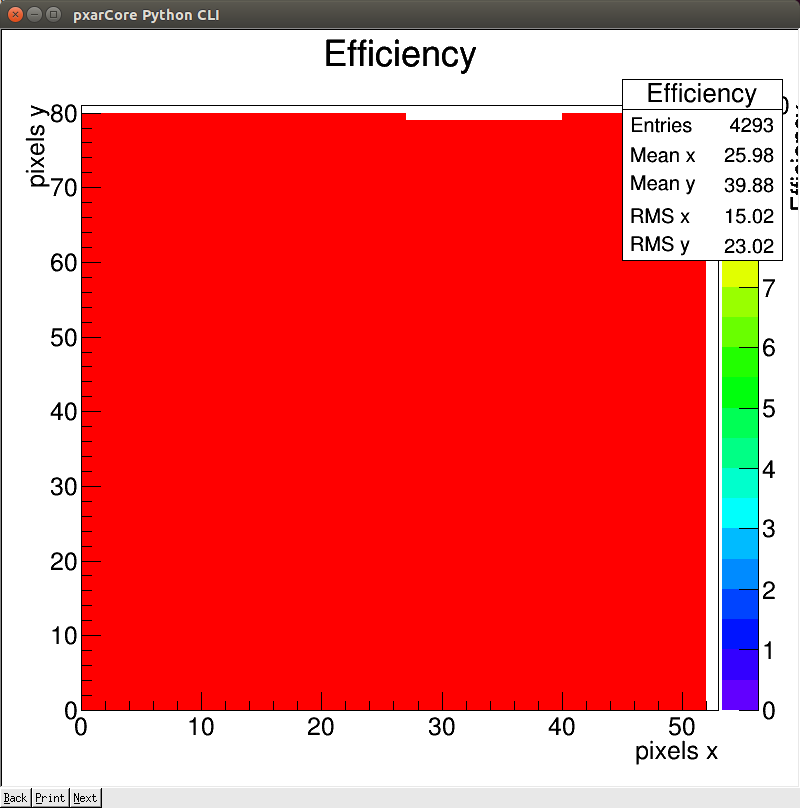
\includegraphics[width=0.47\textwidth]{pixmap}\label{ppixmap}}
	\caption{Two pXar tests.}
	\label{ppxartest}
\end{figure}\no
% ========================================================
\subsection{PixelAlive}
The PixelAlive test shows the efficiency of every pixel for ten readouts, checks if every pixel can be masked and if the address decoding works properly. This test is very powerful to quickly inspect the functionality of the readout. An example for a pixel map is shown in \ar{ppixmap}.
% ========================================================
\subsection{Pretest}
The Pretest is a combination of tests that is meant to find the best set up of the \ac{ROC} for calibration pulses. Up until now all the tests, which were designed for the digital \ac{ROC}, work the same way for the analogue one. For the pretest a modification had to be done.\\
First of all the tests checks weather the chip is programmable be reading the analogue current. If that succeeds it continues by optimising the analogue current to a value of $24\,$mA with an iterative procedure. The analogue current increases very linearly with \textit{vana}. The iteration makes use of the general slope of that rise and was failing for the analogue chip. That is why measuring points of the function iana(vana) were recorded with the python \ac{CLI} utilising the commands:
\begin{itemize}\ubuntu
	\tri setDAC vana <\textit{value}>
	\tri getTBia
\end{itemize}
The slope was then extracted from the points by means of a linear regression. It was found that the slope of the analogue chip is roughly a magnitude of order smaller than for the digital and amounts to a value of roughly $0.5\,$mA/DAC compared to $6\,$mA/DAC for the digital chip. From this fact can be deduced that the analogue resistivity of the two chips has the same ratio as the two slopes. After making the vana subtest dependent on the chip and setting the correct slopes, the test was working for the analogue chip as well.\\
If from a list of ten pixels any can be read out successfully the test proceeds with a DacDacScan and sets \textit{vthrcomp} $50$ \ac{DAC}s below the upper threshold of the tornado plot. For that value of \textit{vthrcomp} caldel is set to a value closest to the middle of the tornade by minimising the distance to either side. Finally all changed \ac{DAC}s are saved to their respective files. 
% ========================================================
\subsection{Trim}\label{strim}
The Trim test was implemented to unify the response of all pixels by putting them to the same threshold. Due to variations in electronics, every pixel has a slightly different threshold until it starts sending pixel signals to the periphery.\\
There are two \ac{DAC}s and the so called trim bits that were designed to unify the threshold: \textit{vthrcomp} sets a global threshold, the trim bits can be set differently for each pixel and lower the threshold in a $4\,$bit range\footnote{$1111=15$ is equivalent to an offset of $0$ and $0000$ is the maximum offset}. The amount each trim bit corrects is set by the \ac{DAC} $vtrim$. The only input parameter of the test is the threshold in \textit{vcal} units that the \ac{ROC} shall be unified to.\\
In a first step the algorithms measures the thresholds\footnote{Speaking of the threshold always refers to an absolute value. The \ac{DAC} \textit{vthrcomp} is actually an inverted unit. So if the threshold is raised \textit{vthrcomp} is decreased} for each pixel with the fixed target \textit{vcal}. This is achieved by raising the threshold until the signal is vanishing. Since the trim bits can only lower the threshold afterwards, the highest of these thresholds is selected and set as a global common threshold (q.v. \ar{ptrimthresh}).\\
Afterwards that \textit{vthrcomp} value is kept constant and the \textit{vcal} value for each pixel is raised until the pixels starts showing a signal. The pixel with the highest \textit{vcal}, which has the biggest deviation from the global threshold, is selected and all its trim bits set to $0$ (q.v. \ar{ptrimvcal}). That lowers the threshold by the biggest possible amount. In order for that value to be the same as the global threshold \textit{Vtrim} is raised until its threshold \textit{vcal} is equivalent to the target  \textit{vcal}.\\
In a last step the trim bits for each pixel are set, s.t. their \textit{vcal} is also equivalent to the target \textit{vcal}.\\
If the test succeeds all pixels are set to uniform threshold. For the beam tests as well as for diamond pixel chips it is desirable to set the threshold very low, to collect as much data as possible. The lowest values that could be achieved with the test from pXar are shown in \ar{ttrim}. The limiting factors are the time walk of the low signals, which take longer to get to the comparator and the electric noise of the pixels.
\begin{table}[ht]
	\centering
	\begin{tabular}{c|c|c}
		\noalign{\hrule height 2pt}
		\textbf{\ac{ROC}}	& \textbf{\textit{vcal$_{\z{min}}$}} 	& 	\textbf{electrons}	\\\hline
		analogue 						& $40$						&	$2600$				\\
		digital							& $28$						&	$1300$				\\
		\noalign{\hrule height 2pt}
	\end{tabular}
	\caption{Minimim vcal and electron threshold achieved by trimming. The conversion factor can be measured using x-rays. }
	\label{ttrim}
\end{table}
\begin{figure}[ht]
	\centering
	\subbottom[Finding the global maximum threshold. In the example it is set to the threshold of the pixel $25\ 31$.]{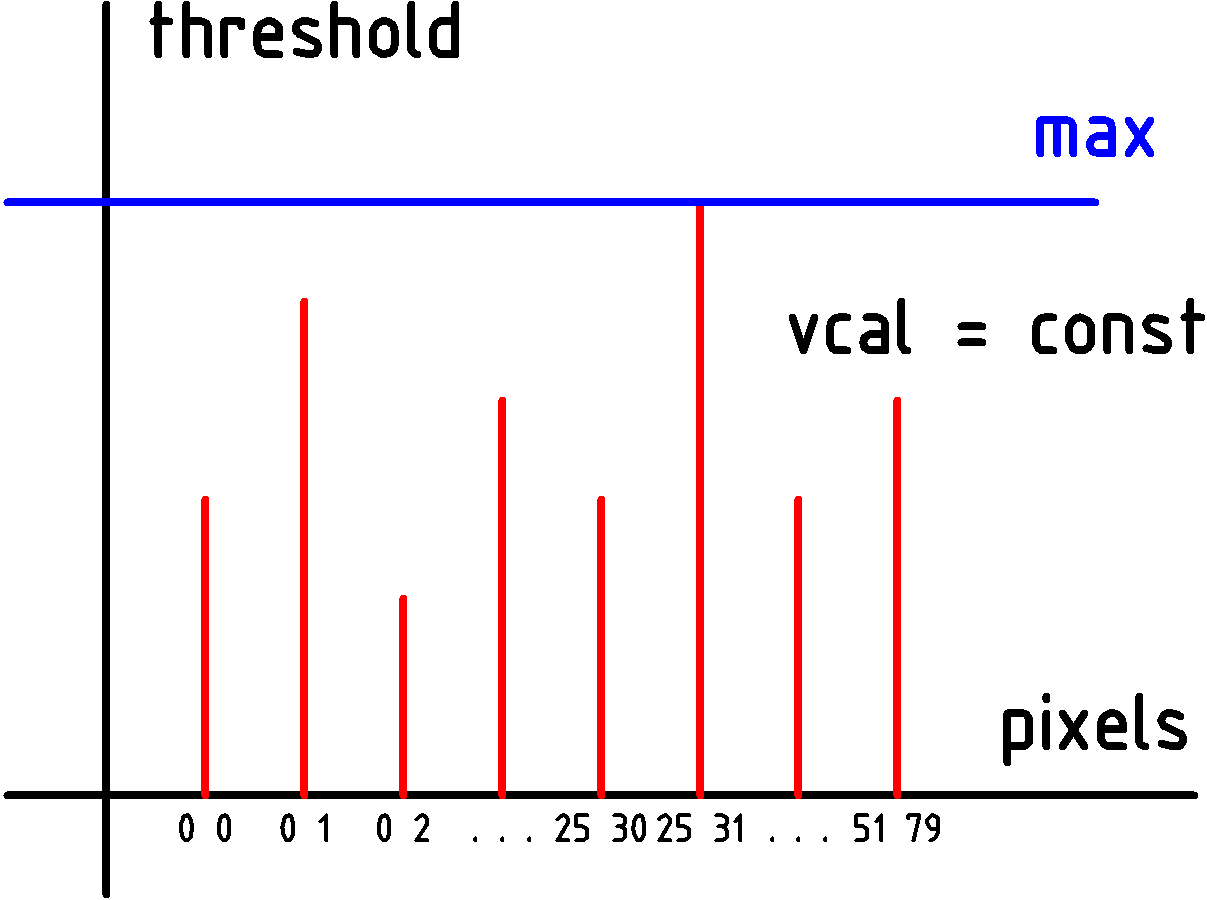
\includegraphics[width=0.47\textwidth]{trimthresh}\label{ptrimthresh}}
	\hfill
	\subbottom[Finding the pixel with maximum difference (in vcal units) to the max threshold. In the example pixel $0\ 2$. ]{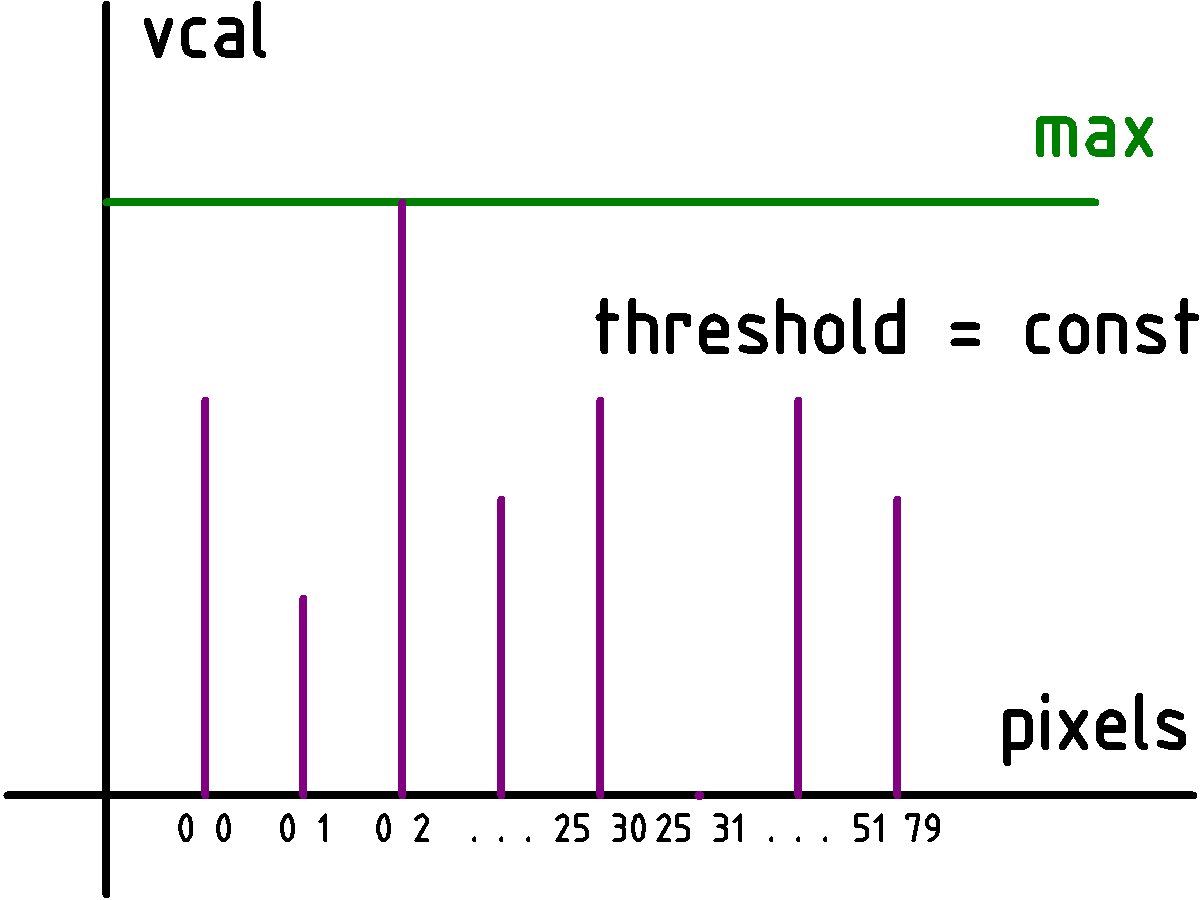
\includegraphics[width=0.47\textwidth]{trimvcal}\label{ptrimvcal}}
	\caption{Visualisation of the trim process.}
	\label{ptrim}
\end{figure}\no
% ========================================================
% FAST-OR
% ========================================================
\section{Fast-OR Dependencies}\label{sfastor}
The fast-OR signal, which is only available for the analogue chips, is used as trigger for all experiments done during this thesis except when using calibrate signals. That is why it is very important to understand its behaviour in terms of signal shape. The three \ac{DAC}s \textit{vsumcol}, \textit{vnpix} and \textit{vicolor} in combination with the number of hits per \ac{DC} and the total number of hit \ac{DC}s determine the shape. For the experiments it is important to collect every single pixel hit, which is why a constant and reliable signal is desirable. The aforesaid \ac{DAC}s are designed for a self triggering mode. \textit{Vnpix} and \textit{vicolor} are meant to set thresholds for minimum number of hits per \ac{DC} and the minimum number of \ac{DC}s with hits.\\ 
In order to measure the fast-OR signal a single analogue \ac{ROC} was connected to a \ac{DTB} and controlled with the python \ac{CLI}. Single calibrates can be sent with the \ac{PG} by utilising the command:
\begin{itemize}
	\tri \ubuntu daqTrigger 1 500
\end{itemize}
In \ar{pfastor} the dependencies for a single activated pixel are demonstrated. Increasing \textit{vsumcol} starting from $0$ results in a decrease of the bump on left side of the pulse and shifts the falling right edge slightly to the left. $6$ has been found as good working point.\textit{Vicolor} showed the same behaviour as \textit{vnpix} during their variation. There are three different states (q.v. \ar{pvnpix}) of the signal that merge into each other upon certain thresholds. Within roughly two units of the \ac{DAC}s one signal is merged into another. At a final threshold the signal vanishes completely. The measured thresholds are shown in \ar{tfastor}. The largest signal has biggest range and is the on that has to be used as signal for the fast-OR. Any value within its range serves, so $99$ and $40$ were chosen for $vicolor$ and $vnpix$ respectively.\par
\begin{table}[ht]
	\centering
	\begin{tabular}{c|c|c}
		\noalign{\hrule height 2pt}
		\multirow{2}{*}{\textbf{Signal}}	& \multicolumn{2}{c}{\textbf{Range}} 	\\\cline{2-3}
											& \textit{vnpix}	& \textit{vicolor}	\\\hline
		large 								& $\wz\wz0-113$		& $34-255$			\\
		middle 								& $114-122$			& $19-\wz33$		\\
		small 								& $123-127$			& $16-\wz18$		\\
		off 								& $127-255$			& $\wz0-\wz15$		\\		
		\noalign{\hrule height 2pt}
	\end{tabular}
	\caption{Thresholds of \textit{vnpix} and \textit{vicolor}}
	\label{tfastor}
\end{table}
\begin{figure}[ht]
	\centering
	\subbottom[Effect of different \textit{vsumcol}]{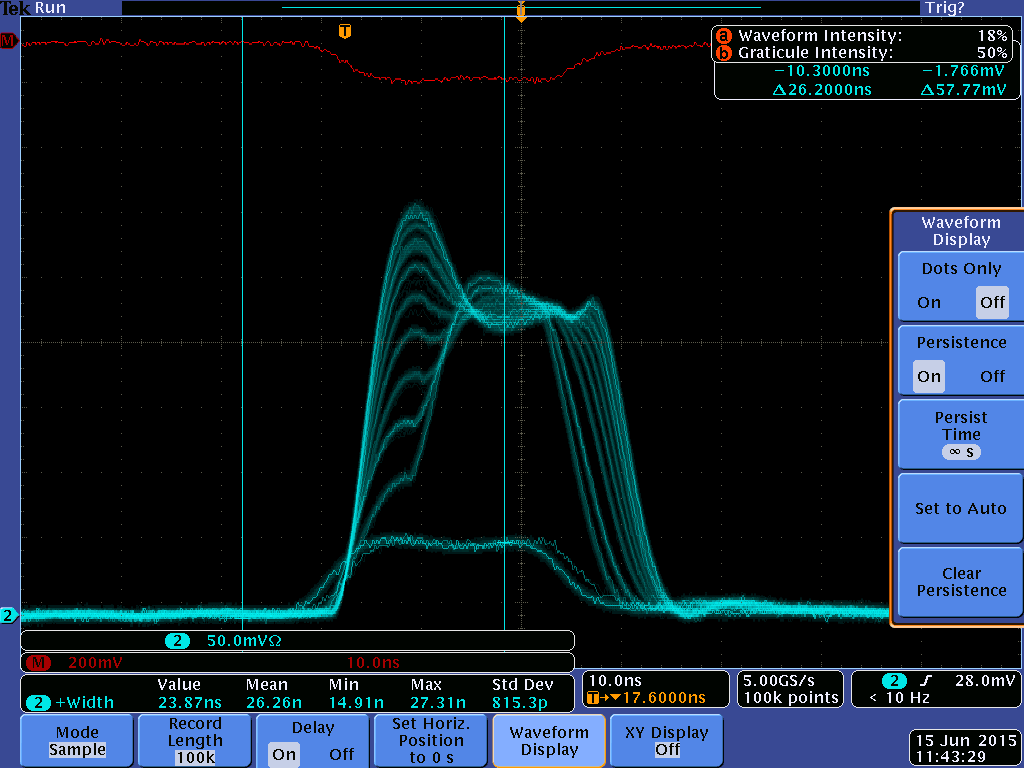
\includegraphics[width=0.47\textwidth]{vsumcol}\label{psumcol}}
	\hfill
	\subbottom[Effect of different \textit{vnpix} and \textit{vicolor}]{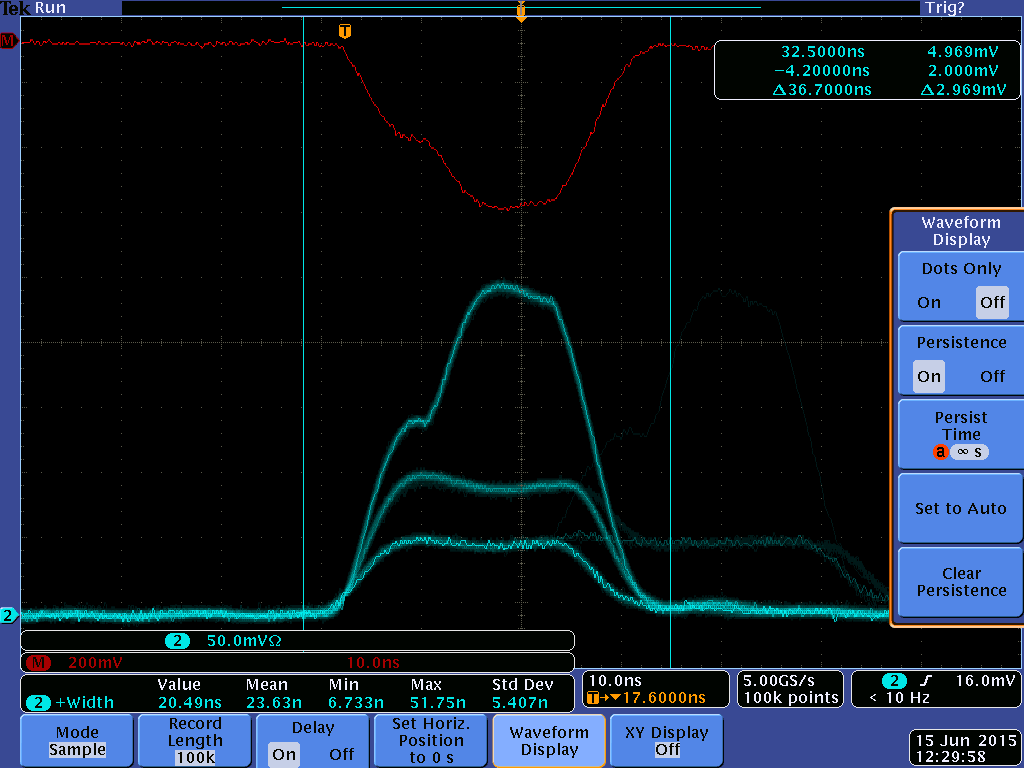
\includegraphics[width=0.47\textwidth]{vnpix}\label{pvnpix}}
	\caption{\ac{DAC} effects on the fast-OR of a single pixel measured with and oscilloscope (blue lines).}
	\label{pfastor}
\end{figure}\no
With the above \ac{DAC} settings the dependencies of the number of hit pixels and hit \ac{DC}s was surveyed and the basic shape of the fast-OR was measured, which is shown in \ar{phitcols}. If only one pixel is activated its position within the \ac{ROC} is completely irrelevant, all signals look like \ar{m1}. A single hit produces a roughly $25\,$ns long pulse with slowly rising edges and a short plateau of about $280\,$mV. It also makes no difference how many pixels within one \ac{DC} are activated or how many consecutive \ac{DC}s were hit, the outgoing signal still looks like a single pixel hit. However, the signal begins to change if more than one non-consecutive\footnote{In this context non-consecutive means that one hit \ac{DC} is followed by a number of non hit \ac{DC}s until another \ac{DC} is hit.} \ac{DC} is hit. If this is the case, a second pulse is slowly rising within the rising edge of the single hit signal. For every additional non-consecutive hit \ac{DC} the bump gets bigger until it gets stable at $11$ hits. The second pulse is merging with the first one which lengthens the overall signal just a few nanoseconds, but increases the rising slope a lot. The signal is aside from that almost independent from the total number of hit pixels Yet when more than approximately $87\,$\% of all pixels were hit, the signal gets more than twice as long and shows a characteristic double peak (q.v. \ar{pallfast}).\\
Since it is very unlikely that almost the whole \ac{ROC} or a large number of non-consecutive \ac{DC} is hit at the same time. The fast-OR signal can be considered very stable and very reliable. It was also verified that the shape of the fast-OR is not changed by the use of either telescope.
\begin{figure}[ht]
	\centering
	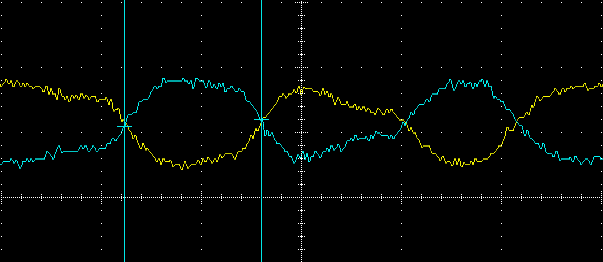
\includegraphics[width=0.52\textwidth]{fastOR/a1}
	\caption{Fast-OR with all pixels activated}
	\label{pallfast}
\end{figure}\no
\begin{figure}[ht]
	\centering
	\subbottom[Single hit pulse, length intersection]{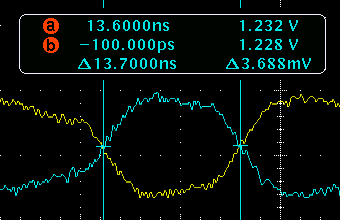
\includegraphics[width=0.31\textwidth]{fastOR/m2}\label{m1}}
	\hfill
	\subbottom[Single hit pulse length]{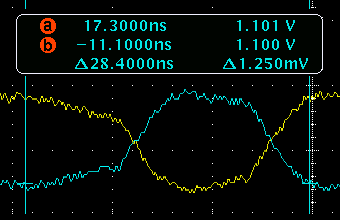
\includegraphics[width=0.31\textwidth]{fastOR/m1}\label{m2}}
	\hfill
	\subbottom[Single hit pulse height]{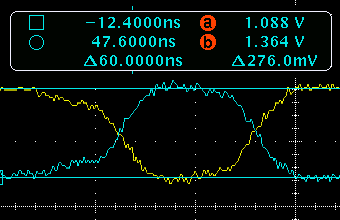
\includegraphics[width=0.31\textwidth]{fastOR/m3}\label{m3}}\\
	\subbottom[1 non-consecutive \ac{DC}s]{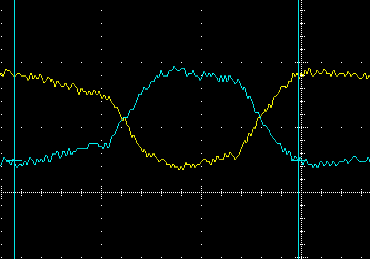
\includegraphics[width=0.31\textwidth]{fastOR/d1}\label{pd1}}
	\hfill
	\subbottom[2 non-consecutive \ac{DC}s]{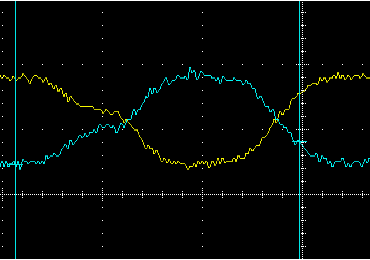
\includegraphics[width=0.31\textwidth]{fastOR/d2}\label{pd2}}
	\hfill
	\subbottom[3 non-consecutive \ac{DC}s]{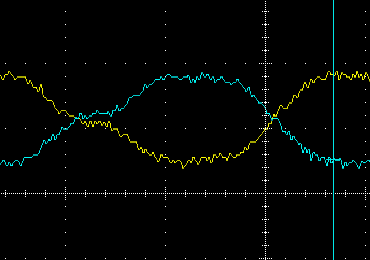
\includegraphics[width=0.31\textwidth]{fastOR/d3}\label{pd3}}\\
	\subbottom[4 non-consecutive \ac{DC}s]{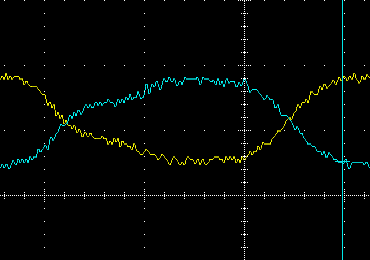
\includegraphics[width=0.31\textwidth]{fastOR/d4}\label{pd4}}
	\hfill
	\subbottom[5 non-consecutive \ac{DC}s]{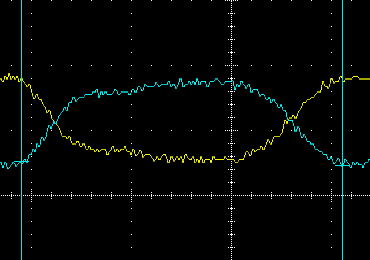
\includegraphics[width=0.31\textwidth]{fastOR/d5}\label{pd5}}
	\hfill
	\subbottom[6 non-consecutive \ac{DC}s]{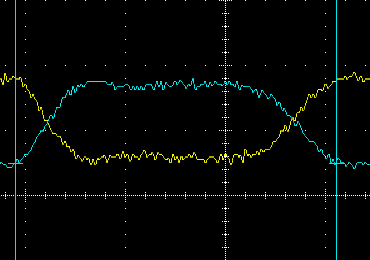
\includegraphics[width=0.31\textwidth]{fastOR/d6}\label{pd6}}\\
	\subbottom[7 non-consecutive \ac{DC}s]{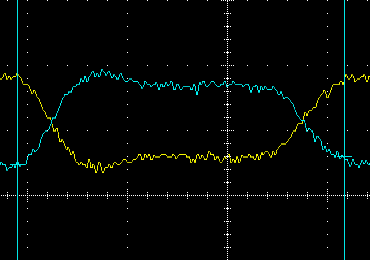
\includegraphics[width=0.31\textwidth]{fastOR/d7}\label{pd7}}
	\hfill
	\subbottom[8 non-consecutive \ac{DC}s]{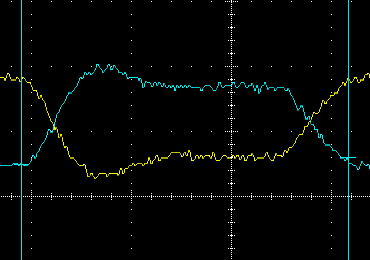
\includegraphics[width=0.31\textwidth]{fastOR/d8}\label{pd8}}
	\hfill
	\subbottom[9 non-consecutive \ac{DC}s]{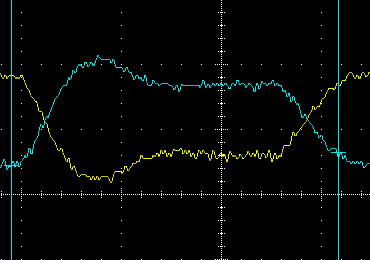
\includegraphics[width=0.31\textwidth]{fastOR/d9}\label{pd9}}\\
	\subbottom[10 non-consecutive \ac{DC}s]{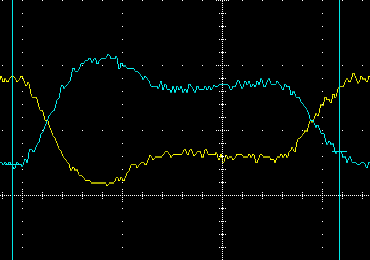
\includegraphics[width=0.31\textwidth]{fastOR/d10}\label{pd10}}
	\hspace*{0.45cm}
	\subbottom[11 non-consecutive \ac{DC}s]{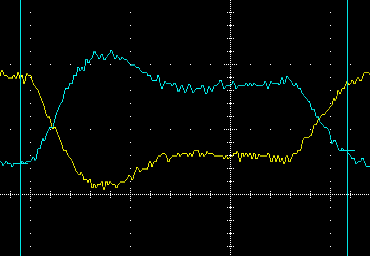
\includegraphics[width=0.31\textwidth]{fastOR/d11}\label{pd11}}
	\caption{Fast-OR dependency on hit pixels and \ac{DC}s measured with an oscilloscope. The blue and the yellow line are the two differential signals of the fast-OR.}
	\label{phitcols}
\end{figure}\no
% ========================================================
% WBC Scan
% ========================================================
\section{WBC Scan}
The \textit{wbc} is a very important value for external triggering. Only if it is set to the exact time in clock cycles that the trigger takes to get to the \ac{ROC} after it was hit the \ac{ROC} will release the hit information. Originally it was very laboriously to find correct value. Using the old telescope every plane was set to a different \textit{wbc} until one of them showed hits in the beam. That is why an easier scan using the python \ac{CLI} was implemented.\\
It could be accomplished using the set-up with a single plane and the the radioactive beta source \chemfig{Sr^{90}} under the application of the trigger logic in \ar{striglog1}. The function 
\ubu{wbcScan [min\_wbc=90] [max\_trig=50] [max\_wbc=130]}
automatically finds the \textit{wbc} for an arbitrary number of chips connected to the \ac{DTB}. It also delivers information about the efficiency of each single chip and the relative phase of the trigger compared to the clock. The values in the square brackets are the arguments with their default values. The functionality of the wbcScan is sketched in the following.\par\vspace*{-5pt}
First of all the trigger source of the \ac{DTB} has to be set to ``extern'' to 
\begin{wrapfigure}{l}{5cm}
	\vspace*{-10pt}
	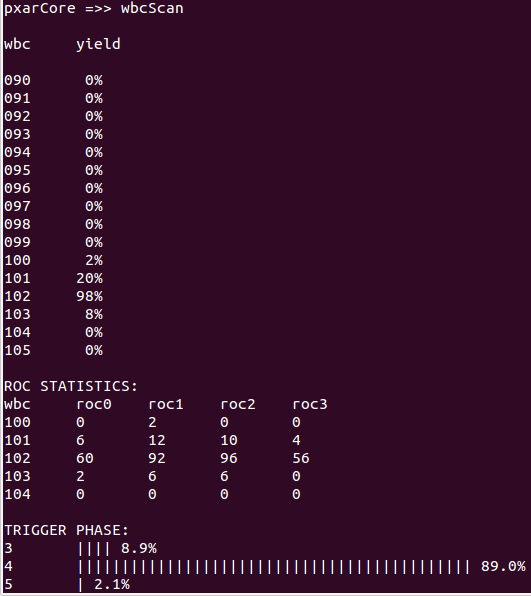
\includegraphics[width=4.9cm]{wbcscan1}
	\caption{Exemplary output of the wbcScan}
	\label{pwbc1}
	\vspace*{-5pt}
\end{wrapfigure} switch to external triggers. Afterwards a new \ac{DAQ} session is started and function starts looping over all \textbf{wbcs} from \textit{min\_wbc}. For every loop it reads out \textit{max\_trig} events and counts the events that have at least one pixel hit in any of the chips (basic yield) as well as the events with at least one pixel hit for every single plane. If the basic yield exceeds $90\,$\% the loop will collect the data for three more \textbf{wbcs} before it stops. Otherwise it will loop over all \textit{wbc}s until \textit{max\_wbc}. After the function is done with looping it will select and set the \textit{wbc} with the highest basic yield and plot a graph with all measured values (q.v. \ar{pwbc2}). In the end it measures the trigger phase for $1000$ events, which is an information the \ac{DTB} acquires via sampling trigger and clock signal with the internal $400\,$MHz clock. Thus, there are $10$ possible phases. Finally it will produce a statistic with the yields per \ac{ROC} some values around the best $wbc$ and a statistic of trigger phases that have more than one event, which is shown in \ar{pwbc1}.
\begin{figure}[ht]
	\centering
	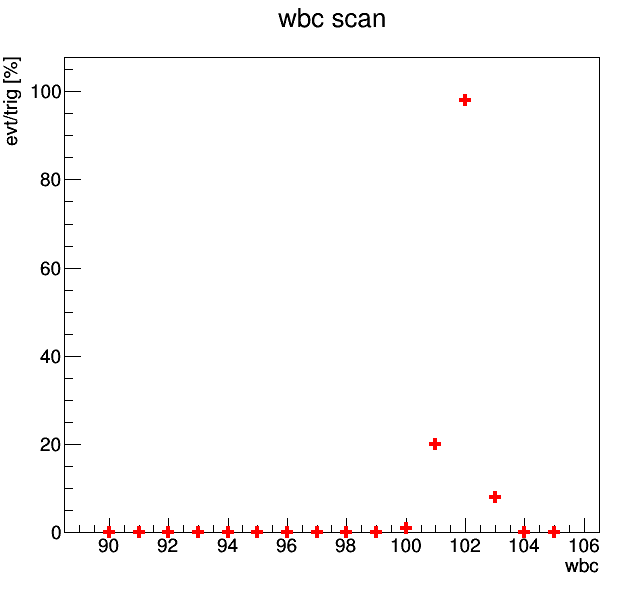
\includegraphics[width=0.6\textwidth]{wbcscan2}
	\caption{Plot of the basic yield of wbcScan}
	\label{pwbc2}
\end{figure}\no
% ========================================================
% DYING FAST-OR
% ========================================================
\section{\ac{TBM} problems}\label{stbmprob}
The software \ac{TBM} is completely controlled by the firmware of the \ac{DTB}. Its basic working principle is describe in \ar{stbm}. During the beam test experiments two problems concerning the \ac{TBM} were encountered that are discussed in the following.
% ========================================================
\subsection{Timing of the \ac{TBM} Trailer}
At the begin of the beam test at \ac{DESY} the data could not be read out at all with the pXar core decoder. Looking at the raw data with the \ac{CLI} revealed that pixels get validated but that the end of the last hit was always cut off after the first level. The events looked like this:
\begin{equation*}
	\overbrace{\hspace*{2.2cm}}^{\z{\ac{ROC} header}}\hspace*{2pt}\overbrace{\hspace*{4cm}}^{\z{\nth{1} pixel hit}}\hspace*{4.3cm}
\end{equation*}
\vspace*{-1.1cm}
\termi{[-205, -8, 36, -2, 54, -46, 148, -4, 78, 103]}
The first thought was an inappropriate toutdelay setting, increasing this delay did not change anything. After that the full raw data blob was investigated showing that the \ac{TBM} header was written in the middle of the last pixel hit. In hexadecimal format that looked like\footnote{Every set of 4 hex numbers is equal to one data word of $16\,$bit}:
\begin{equation*}
	\hspace*{0.5cm}\overbrace{\hspace*{1.9cm}}^{\z{\ac{TBM} header}}\hspace*{2pt}\overbrace{\hspace*{2.9cm}}^{\z{\ac{ROC} header}}\hspace*{2pt}\overbrace{\hspace*{5.9cm}}^{\z{\nth{1} pixel hit}}
\end{equation*}
\vspace*{-1.1cm}
\termi{[a019 8001 8f3e 0006 006e 0fd8 0007 0fd3 00d5 00ad 0092}
\begin{equation*}
	\overbrace{\hspace*{5.9cm}}^{\z{\nth{2} pixel hit}}\hspace*{3.7cm}
\end{equation*}
\vspace*{-1.0cm}
\begin{itemize}
 \item[] \terminal{$\hdots$ 0fd4 e000 c001 0077 0044 409e]} 
\end{itemize}
\vspace*{-0.5cm}
\begin{equation*}
	\underbrace{\hspace*{1.9cm}}_{\z{TBM trailer}}\hspace*{5.7cm}
\end{equation*}
The \ac{TBM} header and trailer both consist out of two words, the first word of the header is initiated with an \textit{a} and the first word of the trailer is initiated with an \textit{e} as shown in the example. These points uses the splitter of pXar to cut the whole data stream into single events, which is why the data is cut off too early in this case.\\
The problem could be temporarily fixed by rewriting the splitting so that it will end the event four positions after it recognised the trailer. Now, the data could be read out with pXar, but a decoding issues arose which is shown in \ar{pdecerr}. Only the last plane of a four plane telescope was showing five vertical stripes within the pixel map. Vertical stripes are caused when the second column address (C1) is set to a constant value. Unfortunately the \ac{TBM} trailer was not only at the wrong position but was overwriting the pixel data as well. In order to avoid the decoding error the last hit of every event had to be discarded.\\
The whole problem could be solved by a new firmware of the \ac{DTB}. Apparently the \ac{ADC} of the \ac{DTB} takes twelve clock cycles to digitise the analogue data. Thereby the data was written to late into the \ac{RAM} even though the \ac{TBM} already started writing the trailer. By taking the delay of the \ac{ADC} into account the whole problem vanished be adding a delay to the \ac{TBM} trailer if the \ac{ADC} is used to digitise the data stream.
\begin{figure}[ht]
	\centering
	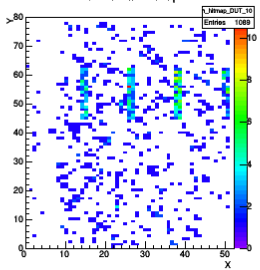
\includegraphics[width=0.5\textwidth]{decodingerr}
	\caption{Decoding error in a pixel plane.}
	\label{pdecerr}
\end{figure}\no
% ========================================================
\subsection{Vanishing Fast-OR}
Later during the same beam test another severe problem was discovered. Using the new firmware of the \ac{DTB} the fast-OR coincidences of two planes in an electron beam were vanishing shortly after starting to take data. Also the single fast-OR showed a decreasing rate.\\
Taking a closer examination at PSI revealed that fast-OR of a single plane is completely vanishing if is self triggered on the signals of a strong radioactive \chemfig{Sr^{90}} source. However, it was only vanishing if the \textit{wbc} is set correctly and the triggers get validated in the \ac{ROC}. If the \textit{wbc} was off the fast-OR remained unchanged. For correct \textit{wbc} the rate of the fast-OR was decreasing stepwise until it went down to zero. The speed of this process is highly dependent on the rate of the passing beta particles. Sometimes the fast-OR starts reviving after going to zero but then vanished again.\\
The explanation for that behaviour is a token trigger mismatch in the \ac{ROC} periphery and could be verified by a simple experiment. While putting a strong source on top the analogue chip a high rate of random triggers (without tokens) were sent with the \ac{PG}. Due to the high rate of betas and triggers it happens that some triggers coincidentally come at the right \textit{wbc} and validate a hit, which causes the \ac{DC} to freeze. Since there is no token or no reset to free the \ac{DC}, it just remains frozen and will stop sending fast-ORs. Depending on the rate of trigger and source a stepwise decrease of rate can be observed.\\
In order to find out what is causing the mismatch in self-triggering mode, the signals \textit{token in, token out}, \textit{ctr} of the \ac{DTB} and the fast-OR itself were investigated closer. The first three can be made accessible via
\ubu{signalProbe  <\textit{output}> <\textit{signal}>\footnote{Output stands for the LEMO output of the \ac{DTB} (d1, d2, a1, a2) and the signals are tin (token in), tout (token out) and ctr. }}
In some occasions there were two or more tokens for a single trigger. Such an event is shown in \ar{p2tok}. That is exactly what causes the mismatch of the token and trigger count on the \ac{ROC} and vanishing fast-OR. Since the trigger and token counter are $4\,$bit numbers it is possible that they get back in sync after a while, which explains the revival.\\
The reason for that could be found inspecting the internal signals of the \ac{DTB} even further. It is possible to send almost every signal that used by the \ac{FPGA} so a pin on the \ac{PCB} of the \ac{DTB} where they can be read out with a digital probe of an oscilloscope. By looking at the internal asynchronous trigger signal, which is a logic signal made from external trigger input of the \ac{DTB}, it was conspicuous that the signal was too long in some occasions. Usually it should be exactly one clock cycle but every time multiple token showed up, this signal was lengthened by the amount of additional tokens. Both the asynchronous trigger and the token in are sampled with internal signals called start and stop. These signal are identical and are generated via the internal $400\,$Mhz and $80\,$Mhz clocks and are shown in \ar{pstop}. The asynchronous trigger is generated if the external trigger that is sent to the \ac{DTB} coincides with the start signal and is stopped with any stop signal, which why it should be exactly one clock cycle long. For every time the start signals coincides with the asynchronous trigger the \ac{TBM} sends a token. So if the asynchronous signal is longer than one clock cycles multiple tokens are sent.\\
By looking at stop signal the main cause for the whole problem could be found. It was not continuous but sometimes single pulses were just missing. If a single pulse was missing when the asynchronous trigger should be stopped, the trigger gets too long and is stopped at the next available stop pulse, shown in \ar{ptriglong2}.\\
The solution was lying in the generation of the stop/start signal, which was done if both clocks have a positive edge. If the clock would just go minimal out of sync it could happen, that this operation would not work. By fixing that signal, the whole problem could be solved.
\begin{figure}[ht]
	\centering
	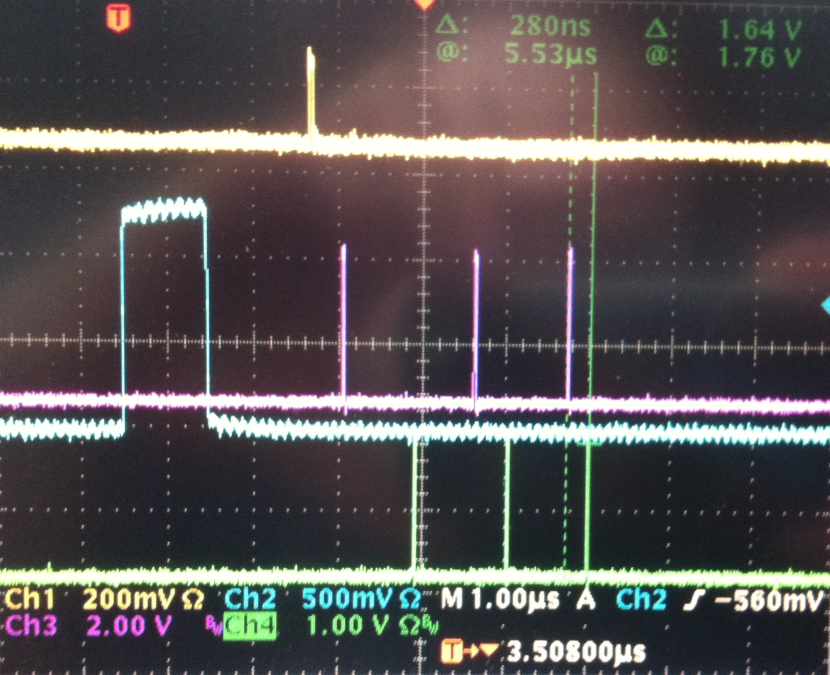
\includegraphics[width=0.6\textwidth]{doubletoken}
	\caption{Measurement of the signals: \ac{CTR} (yellow), discriminated fast-OR (cyan), token in (magenta), token out (green)}
	\label{p2tok}
\end{figure}\no
\begin{figure}[ht]
	\centering
	\subbottom[Generation of the start/stop signal.]{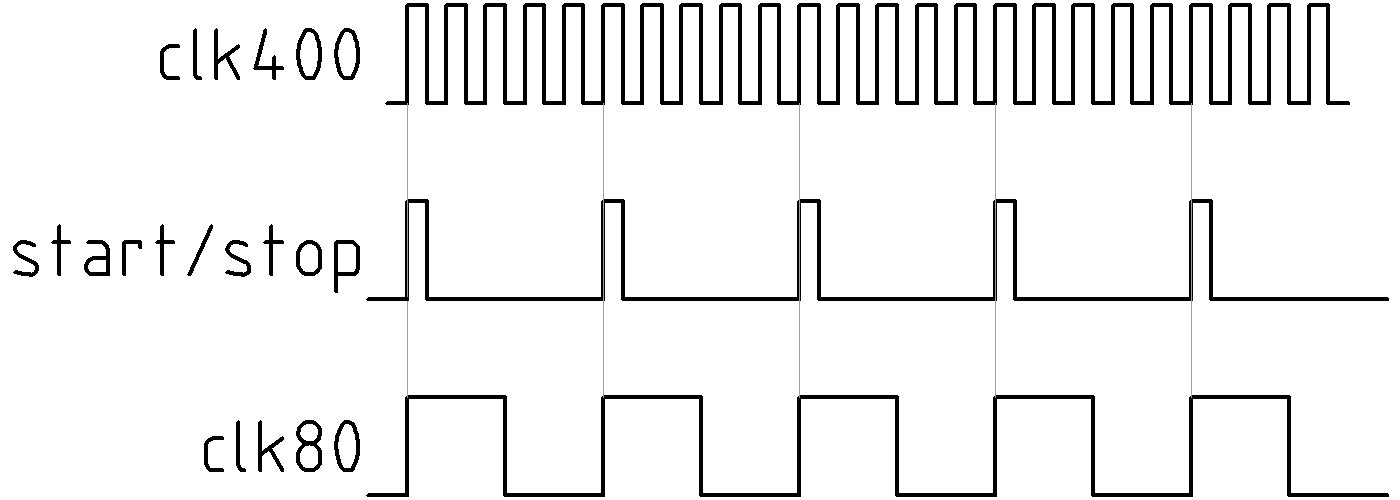
\includegraphics[width=0.6\textwidth]{stopsig}\label{pstop}}\\
	\subbottom[Functioning asynchronous trigger.]{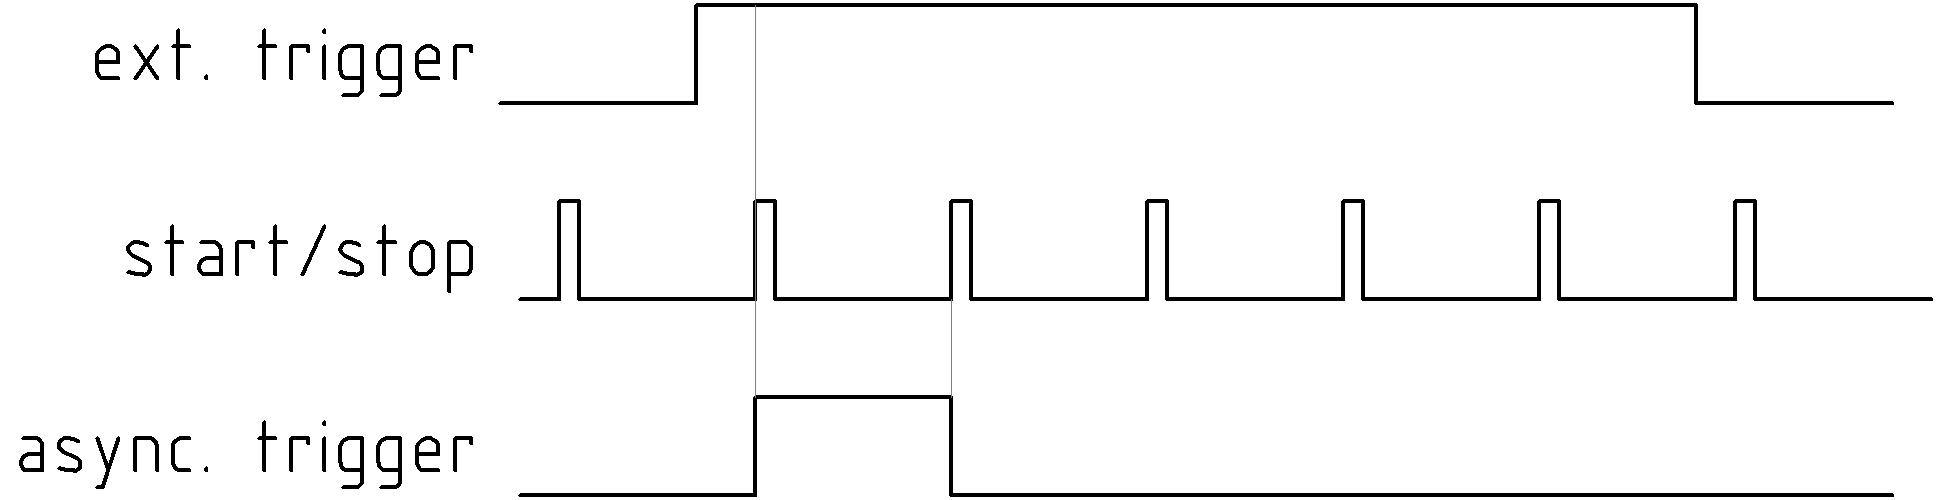
\includegraphics[width=0.8\textwidth]{triglong1}\label{ptriglong1}}\\
	\subbottom[Too long asynchronous trigger.]{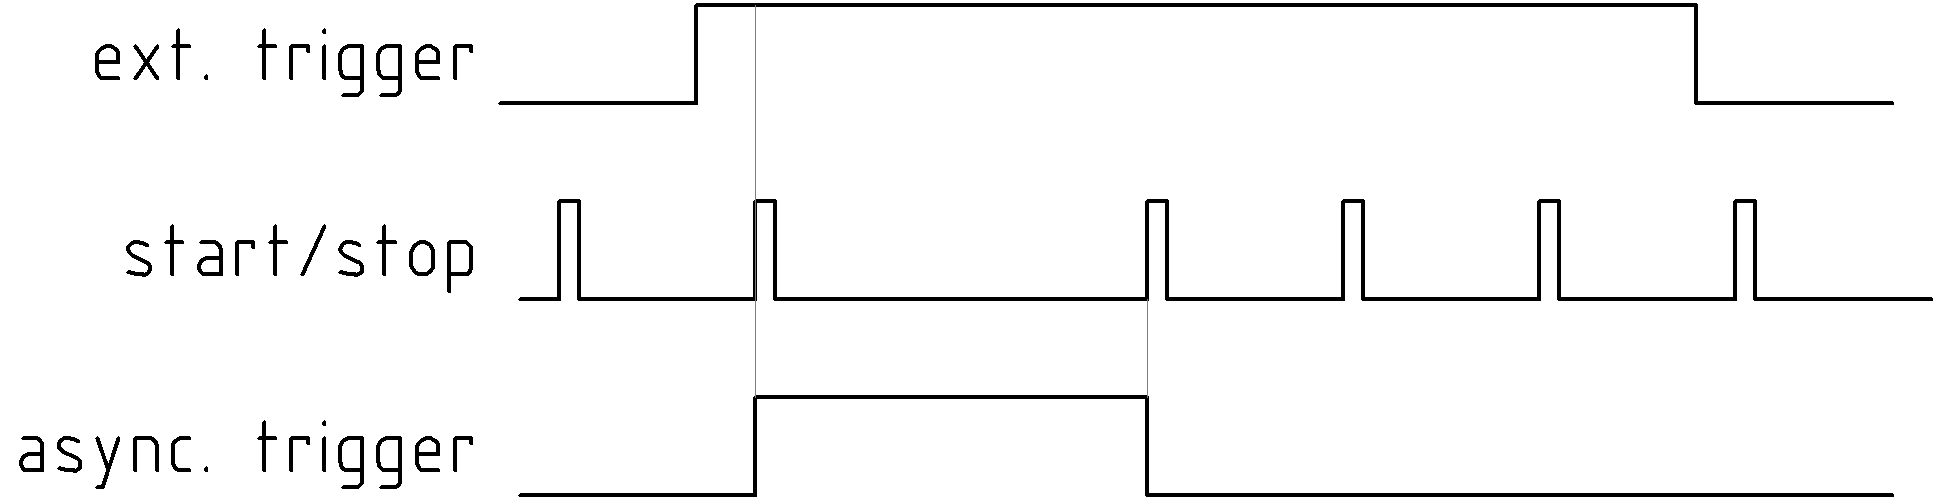
\includegraphics[width=0.8\textwidth]{triglong2}\label{ptriglong2}}\\
	\caption{\ac{DTB} signals}
	\label{psigdtb}
\end{figure}\no
% ========================================================
% CLI TESTS
% ========================================================
\section{\ac{CLI} Test Implementations}
% ========================================================
% DIA SHADOW
% ========================================================
\section{Finding \ac{DUT} Shadows}
For using diamond pad detectors as \ac{DUT}s it is
\begin{wrapfigure}{r}{5cm}
	\vspace*{-10pt}
	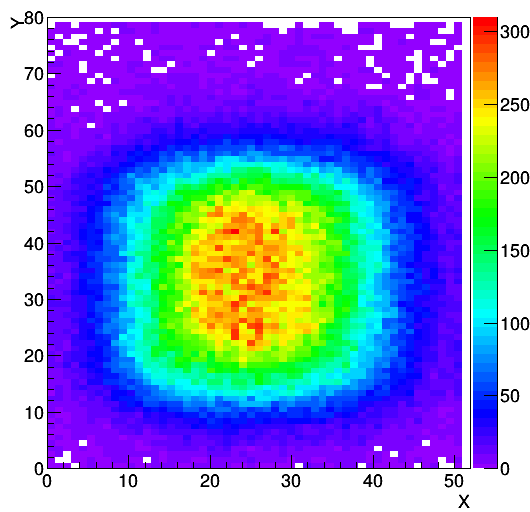
\includegraphics[width=4.9cm]{diashadow}
	\caption{The hit map of analogue pixel plane while triggered on the signal of a diamond pad.}
	\label{pdiashodow}
	\vspace*{-5pt}
\end{wrapfigure} 
important to spatially align the pads, which are only $4\times4\,$mm, within the planes of the telescopes. The following method describes how that can be accomplished.\\
For the method to work at all, the pads have to roughly aligned to the \ac{ROC}s by eye, s.t. at least a tiny fraction of them overlaps relatively to the beam. Then the trigger output of the a DRS4 evaluation board, which is connected to the pads, is used as external trigger for the telescope planes. The DRS4 has to be set up, s.t. it triggers on one of the channels the pads are connected to. With that trigger the wbcScan has to be used to find the correct wbc for the planes. Finally, data can be collected with the telescope that only shows events where the pad had a signal that triggered the DRS4. The result is shown in \ar{pdiashodow}.\\
Using this method, the pad can be placed very accurately relative to the pixel planes. It can be applied for any \ac{DUT} that can be triggered on.
% ========================================================
% OPTIMISE TRIG WINDOW
% ========================================================
\section{Optimisation of the Trigger Window}
% ========================================================
% EUDAQ AND TLU
% ========================================================
\section{Implementation of EUDAQ and \ac{TLU}}
EUDAQ is a data-taking software that is perfect for handling several, independent data streams and aligning them into single events. It was adapted for a beam test set-up for the telescope by the CMS group at \ac{ETH}.
The general beam test configuration was running on three computers and is sketched in the following:
\begin{itemize}
	\item A laptop inside the beam area was running:
		\begin{itemize}
			\item a DRS4 producer, which handles the data and the configuration of a DRS4 board
			\item a cmspixel producer, which handles the configuration the and data of a \ac{DTB}, using the pXar core libraries
			\item a \ac{TLU} producer, which handles the configuration of the \ac{TLU} 
		\end{itemize}
	\item An accessible computer for data-taking running:
		\begin{itemize}
			\item the Run Control
			\item the Logger
		\end{itemize}
	\item A data server for saving the data running:
		\begin{itemize}
			\item the Data Collector
		\end{itemize}
\end{itemize}
Depending on which \ac{DUT}s are to be examined, the configuration of the producers connected to the laptop may vary.
% ========================================================
\subsection{Masking}\label{smasking}
Masking is a very important feature for the CMS pixel detectors. A masked pixel will not send any information to the periphery of the \ac{ROC}. Not only the noisy or malfunctioning pixels can be disabled but it is very powerful to control the effective trigger area. That means by masking certain areas of the pixels chips it is possible to use only triggers of specific position or arrangement of pixels. That is, for example, very useful if \ac{DUT}s with smaller areas than the pixel chip are examined.\\
For that reason masking was implemented into the cmspixel producer using the commands from the pXar core library. Each pixel of each pixel may be masked by reading in a configuration file that has to contain the information shown in \ar{tmask}. An example of a masked area of a pixel chip is shown in \ar{pmask}.
\begin{figure}[ht]
	\centering
	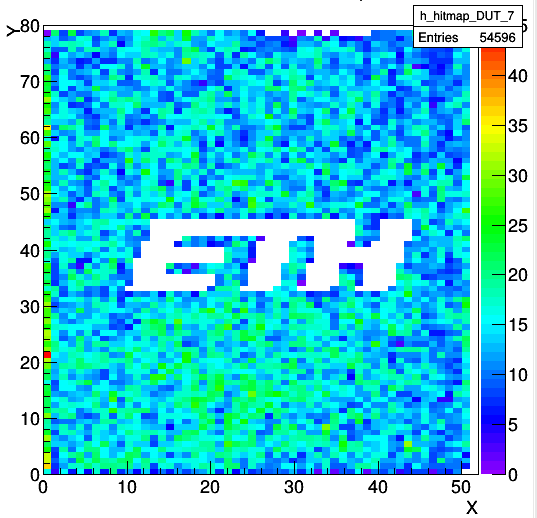
\includegraphics[width=0.6\textwidth]{mask}
	\caption{Example of partly masked pixel chip, the pixels in white area are masked and thus do not send any hits.}
	\label{pmask}
\end{figure}\no
\begin{table}[ht]
	\begin{tabularx}{\textwidth}{l|c|c|c|X}
		\noalign{\hrule height 2pt}
		\textbf{name}	&		\textbf{I2C}		&		\textbf{col}			&		\textbf{row}		&	\textbf{explanation}						\\\hline
		pix		&	$	0	$	&	$	12	$	&	$	36	$	&	mask pixel in col 12 and row 36 of I2C 0			\\	
		row		&	$	1	$	&	$	10	$	&	$	20	$	&	mask row 10-20 (including 10 and 20) of I2C 1		\\
		row		&	$	2	$	&	$	10	$	&	$	10	$	&	mask row 10 of I2C 2								\\
		col		&	$	3	$	&	$	14	$	&	$	30	$	&	mask col 14-30										\\
		roc		&	$	4	$	&				&				&	mask the whole ROC of I2C 4							\\
		cornBot	&	$	0	$	&	$	\wz5$	&	$\wz7	$	&	\multirow{2}{7.5cm}{leaves a box with the lower left corner (5/7) to the upper right corner (12/10) unmasked, i.e. row col 5-12 and row 7-10.}	\\
		cornTop	&	$	0	$	&	$	12	$	&	$	10	$	&														\\
		&&&&\\
		\noalign{\hrule height 2pt}
	\end{tabularx}
	\caption{Examplary masking commands.}
	\label{tmask}
\end{table}
% ========================================================
% PULSE HEIGHT CAL
% ========================================================
\section{Pulse Height Calibration}\label{spulseheight}
In order to draw conclusions about the energy of the particles that pass through the detector, the number of created electron-hole pairs is required. Utilising the information of the GainPedestal test of \ar{sgainped} the pulse height vs. \textit{vcal} points are fitted with an error function using ROOT.
\begin{itemize}
	\item[] $[3]^{*}(\z{TMath}::\z{Erf}((x-[0])/[1]+[2])$
\end{itemize}
The error function is converging very well as shown for two examples in \ar{perrfit}. The fit parameters are saved for every \ac{ROC}. With the conversion factor of the vcal into electrons one is able to convert every every measured pulse height into a number of electrons using these fit functions.
\begin{figure}[ht]
	\centering
	\subbottom[Pixel 14 14]{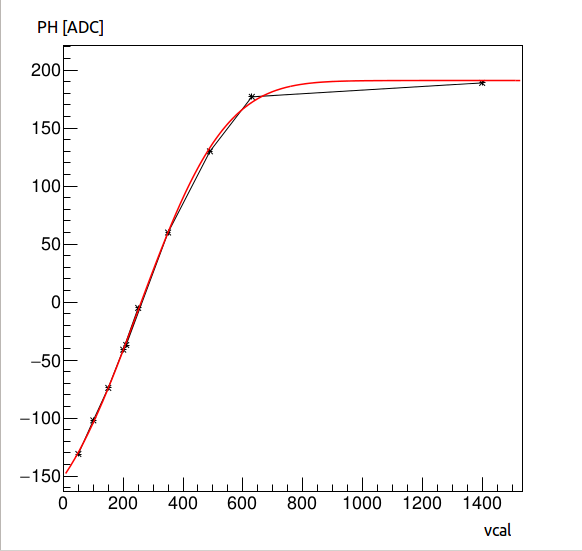
\includegraphics[width=0.47\textwidth]{errfit1}\label{perrfit1}}
	\hfill
	\subbottom[Pixel 26 51]{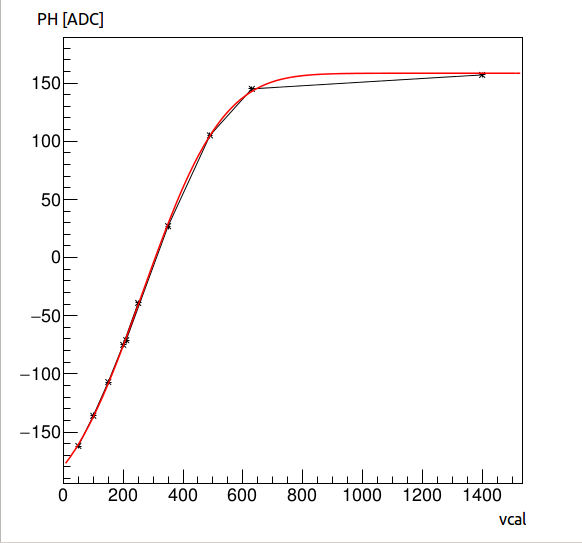
\includegraphics[width=0.47\textwidth]{errfit2}\label{perrfit2}}
	\caption{Fits of the pulse height vs. \textit{vcal} function for two random pixels.}
	\label{perrfit}
\end{figure}\no
% ========================================================
